%!TEX encoding = UTF8
%!TEX root =notes.tex

\chapter{Nombre dérivé}

Le but de ce chapitre est de traiter de la partie \og Variation instantanée, variation globale \fg~du bulletin officiel.

Les capacités attendues sont les suivantes.
\begin{itemize}
	\item Interpréter le nombre dérivé dans le cadre d'un modèle d'évolution.
	\item Interpréter géométriquement le nombre dérivé comme coefficient directeur de la tangente.
	\item Décrire les variations d'un phénomène en mobilisant la dérivée d'une fonction.
	\item Déterminer le sens de variation d'une fonction polynomiale de degré inférieur ou égal à troie (la forme factorisée de la dérivée pourra être donnée).
	\item Prévoir l'évolution d'un phénomène grâce à l'étude de la dérivée d'une fonction.
\end{itemize}

\section{Introduction : calcul de vitesse}

Supposons qu'une voiture roule sur une route droite, qu'on modélise par un point évoluant sur une axe.
En tout temps $t$, on peut connaitre sa position, qu'on appelle $f(t)$.
La voiture n'avance pas à vitesse constante ;
elle peut même s'arrêter pendant un certain temps, ou reculer.

\qs{}{
	Comment calculer la vitesse $V(t)$ de la voiture en tout temps $t$ ?
}{}

Il semble qu'on ait assez d'information pour calculer la vitesse de la voiture, mais que la définition même de la vitesse n'est pas claire.
En physique, on calcule une vitesse moyenne grâce à deux positions en deux temps différents.

	\begin{align}
		v = \dfrac{f(t_2) - f(t_1)}{t_2-t_1}. \label{eq:3.1}
	\end{align}

C'est faisable ici bien sûr, mais cela ne répond pas à la question : la vitesse $V(t)$ qu'on souhaite calculer est la vitesse en un temps $t$ donné, et un seul.
C'est la vitesse \emph{instantanée} de la voiture --- celle qu'on lit sur le tachymètre d'une voiture.


Avant de commencer l'étude, dessinons d'abord quelques situations qui peuvent subvenir.
D'abord, la notation $t$ et $f(t)$ n'est pas anodine : la position de la voiture est une fonction de temps (car à chaque temps est associé une unique position), et on peut la représenter dans un graphique comme ci-dessous.

\begin{tikzpicture}
\begin{axis}[xmin = 0, xmax=5, grid = none,  xlabel={$t$}, ylabel={$f(t) = \sin(90t)$}]
	\addplot[domain=0:5, samples=500] {sin(90*x)};
\end{axis}
\end{tikzpicture}

De l'expression de la vitesse de l'équation \eqref{eq:3.1}, et en prenant $t_1 < t_2$, on remarque trois cas de figure.
\begin{enumerate}
	\item Lorsque la position $f(t)$ augmente, la vitesse $V(t)$ est positive. 
	C'est le cas où la voiture avance.
	\item Lorsque la position $f(t)$ est constante, la vitesse $V(t)$ est nulle.
	C'est le cas où la voiture est immobile. 
	\item Lorsque la position $f(t)$ diminue, la vitesse $V(t)$ est négative.
	C'est le cas où la voiture recule.
\end{enumerate}
Le signe de la vitesse de la voiture est donc liée aux variations de sa position $f(t)$.
Un tableau permet de regrouper les informations obtenues jusqu'ici.
	
\begin{tikzpicture}
	\tkzTabInit
	 %[lgt=3,espcl=1.5]
	 [lgt=5]
       		{$t$ / 1 , Variation de $f(t)$ / 2, Signe de $V(t)$ / 1}
       		{0,1,3,5}
	\tkzTabVar
		{-/0,+/1,-/-1,+/1}
		
	\tkzTabLine
		{,+,t,-,t,+}
\end{tikzpicture}

Comme la vitesse est, par définition, une distance sur un temps, une façon de calculer la vitesse de la voiture en $t_1=4$ est de considérer la position de la voiture légèrement après $4$.
Le choix du pas de temps, qu'on notera $h$, semble cependant important. Posons $t_2 = 4+h$.
Plus le pas est petit, plus la valeur calculée semble intuitivement s'approcher de la vitesse instantanée au temps $t=4$.

La formule de la vitesse de l'équation \eqref{eq:3.1} donne les ratios suivants à calculer avec l'expression $f(t) = \sin(90t)$.
\begin{align*}
	v_{h=1} &= \dfrac{f(5) - f(4)}{5-4} = 1 & v_{h=0,9} &=  \dfrac{f(4,9) - f(4)}{4,9-4} = 1,097 \\
	v_{h=0,8} &=  \dfrac{f(4,8) - f(4)}{4,8-4} = 1,188 & v_{h=0,7} &=  \dfrac{f(4,7) - f(4)}{4,7-4} = 1,272 \\
	v_{h=0,6} &=  \dfrac{f(4,6) - f(4)}{4,6-4} = 1,348 & v_{h=0,5} &=  \dfrac{f(4,5) - f(4)}{4,5-4} = 1,414 \\
	&\dots & &\dots
\end{align*}
On pourra comparer à l'aide de la calculatrice la valeur de $v_{h}$ lorsque $h$ est de plus en plus petit (p.ex. $0,1$ puis $0,01$) à $\frac\pi2$ pour se douter qu'une certaine converge occurre...

\qs{}{
	La vitesse moyenne de la voiture entre $t=4$ et $4+h$ approche-t-elle une certaine valeur qu'on peut déterminer lorsque $h$ tend vers $0$ ?
}{}

Pour répondre à cette question, il s'agit d'interpréter les vitesses calculées graphiquement et de voir ce qu'on obtient lorsque le pas devient nul.

Considérons les points $A$ et $B$ d'abscisses respectivement $t_1$ et $t_2$ sur $\C_f$.
La propriété fondamentale nous dit que l'ordonnée des points est l'image de leur abscisse.
C'est-à-dire que $y_A = f(x_A) = f(t_1)$, et $y_B = f(t_2)$.

L'équation \eqref{eq:3.1} est donc équivalente à
	\[ \dfrac{y_B - y_A}{x_B - x_A}, \]
qui est exactement la formule du coefficient directeur de la fonction affine passant par $A$ et $B$.
Rappelons que le coefficient directeur mesure la pente d'une fonction affine, et que le signe de celui-ci donne les variations de celle-ci.
On répète en fait la même chose en langage affine : si le coefficient directeur est positif, c'est que la vitesse moyenne est positive, et donc que la fonction augmente.

\begin{tikzpicture}
\begin{axis}[xmin = 0, xmax=5, ymin=-1.25, ymax=1.25, grid = none,  xlabel={$t$}, ylabel={$f(t)$}]
	\addplot[domain=0:5, samples=500, myb, thick] {sin(90*x)};
	\addplot[domain=3:5, samples=2, myr] {x-4};
\end{axis}
\end{tikzpicture}
\begin{tikzpicture}
\begin{axis}[xmin = 0, xmax=5, ymin=-1.25, ymax=1.25, grid = none,  xlabel={$t$}, ylabel={$f(t)$}]
	\addplot[domain=0:5, samples=500, myb, thick] {sin(90*x)};
	\addplot[domain=3:5, samples=2, myr] {.9876/.9*(x-4)};
\end{axis}
\end{tikzpicture}
\begin{tikzpicture}
\begin{axis}[xmin = 0, xmax=5, ymin=-1.25, ymax=1.25, grid = none,  xlabel={$t$}, ylabel={$f(t)$}]
	\addplot[domain=0:5, samples=500, myb, thick] {sin(90*x)};
	\addplot[domain=3:5, samples=2, myr] {.95105/.8*(x-4)};
\end{axis}
\end{tikzpicture}
\begin{tikzpicture}
\begin{axis}[xmin = 0, xmax=5, ymin=-1.25, ymax=1.25, grid = none,  xlabel={$t$}, ylabel={$f(t)$}]
	\addplot[domain=0:5, samples=500, myb, thick] {sin(90*x)};
	\addplot[domain=3:5, samples=2, myr] {.89100/.7*(x-4)};
\end{axis}
\end{tikzpicture}


\dfn{Dérivation ponctuelle}{
	Soit $f$ une fonction position suffisamment lisse.
	On calcule, au temps $t$, la vitesse instantanée en considérant
		\[ v_h = \dfrac{f(t+h)-f(t)}{h}, \]
	et en laissant $h$ tendre vers $0$.

	On appelle la valeur limite de $v_h$ la \emph{dérivée ponctuelle} de $f$ au temps $t$.
}{}

\section{Dérivation}

\dfn{Fonction dérivée}{
	Soit $f$ une fonction sur $\R$ suffisamment lisse.
	On définit $f'$, la \emph{fonction dérivée} de $f$, telle que $f'(t)$ soit la dérivée ponctuelle de $f$ en $t$.
}{}

\thm{Linéarité de la dérivée}{
	Soient $f, g$ deux fonctions dérivables sur $\R$, et $\kappa\in\R$ un nombre réel quelconque. 
	Alors
		\begin{enumerate}
			\item $(f+g)' = f' + g'$ ; et
			\item $(\kappa f)' = \kappa f'$.
		\end{enumerate}
}{thm:lin-der}

\mprop{Dérivée des monômes usuels}{
	\centering
	\begin{tabular}{|c|c|}\hline
		Monôme & Dérivée \\ \hline
		$1$ & $0$ \\ \hline
		$x$ & $1$ \\ \hline
		$x^2$ & $2x$ \\ \hline
		$x^3$ & $3x^2$ \\ \hline
	\end{tabular}
}{prop:der-mono}

\thm{Signes et variations}{
	Soit $f$ une fonction dérivable sur $\R$ et $I$ un intervalle quelconque.
	Alors
		\begin{center}
			$f$ est croissante sur $I$ \qquad $\iff$ \qquad $f'$ est positive sur $I$. 
		\end{center}
}{}
